\documentclass{VUMIFPSkursinis}
\usepackage{algorithmicx}
\usepackage{algorithm}
\usepackage{algpseudocode}
\usepackage{amsfonts}
\usepackage{amsmath}
\usepackage{bm}
\usepackage{caption}
\usepackage{color}
\usepackage{float}
\usepackage{graphicx}
\usepackage{listings}
\usepackage{subfig}
\usepackage{wrapfig}

% Titulinio aprašas
\university{Vilniaus universitetas}
\faculty{Matematikos ir informatikos fakultetas}
\department{Programų sistemų katedra}
\papertype{Kursinis darbas}
\title{Laikinų sutrikimų poveikio sesijų valdymo algoritmui tyrimas}
\titleineng{Impact of temporary failures on session management algorithm}
\author{Mantas Petrikas}
\supervisor{doc. Karolis Petrauskas}
\date{Vilnius – \the\year}

% Nustatymai
% \setmainfont{Palemonas}   % Pakeisti teksto šriftą į Palemonas (turi būti įdiegtas sistemoje)
\bibliography{bibliografija}

\begin{document}
\maketitle

\tableofcontents

\sectionnonum{Įvadas}
\subsubsection*{Tyrimo objektas}

  Šiame darbe analizuojamas algortimas, skirtas asinchroniškai valdyti sesijų komunikaciją tarp skirtingu paskritytos sistemos grupių (angl. ,,clusters'') \cite{petrauskas2018asynchronous, petrauskas2019effectiveness}.
  Algoritmas aprašytas TLA\textsuperscript{+} specifikavimo kalba \cite{lamporttla+}, jo korektiškumas yra tikrinamas atviro kodo ,,TLA\textsuperscript{+} toolbox'' įrankiu  \cite{kuppe2019tla+}.

\subsubsection*{Darbo aktualumas}
  
  Moderios didelio praleidumą turinčios sistemos apdoroja tukstančius, ar net milijonus užklausų vienu metu, ir greitai ir patikimai gražinti duomenis.
  Kad efektyviai pasiekti rezultatus, sistemos projektuojamos numatant galimę plėsti jas didiant serverių skaičių ir paskirstant apkrovą tarp jų \cite{soni2016nginx}.
  
  Paskirstytos sistemos suteikia turi daug privalumų - 
  padidėja sistemos prieinamumas, sumažinamas nekritinių sistemos dalių poveikis visos sistemos veiklai,
  suteikiama galimybė didinti sistemos pralaidumą paralelizuojant ir horizontaliai plečiant sistemos resursus. 
  Tačiau paskirstytos sistemos turi ir minusų. Dauguma paskirstytų sistemų problemų susiję su sudėtingesne infrastrukūra ir diegimu (ang. deployment), 
  sistemos būsėnos valdymu ir  vientisumo išlaikymu visose sistemos dalyse \cite{thones2015microservices}.
  Norinti išlaikyti didelį sistemos pasiekiamumą ir operacijų greitumą, dalis sistemų naudoja asynchoninis bendravimą tarp skirtingų sistemų dalių, 
  užtikrinant tik galutinį būsenos nuoseklumą (ang. eventual consistency) \cite{vogels2009eventually}.


  TLA\textsuperscript{+} yra formali, predikatų logiką paremta, aukšto lygio modeliavo kalba, leidžianti projektuoti, aprašyti ir tikrinti sistemų korektiškumą \cite{kuppe2019tla}.
  Ši kalba yra naudojama didžiosiose kompanijose, ,,Intel'' \cite{batson2002high} ,,Amazon'' komponijoje \cite{newcombe2015amazon}, Microsoft ir kitose. 
  Specifikavimo kalba leidžia naudojant predikatų logiką aprašyti pradinę sistemos būseną,
  leistinus sistemos būsenos pakitimus ir savybės kurias modelis turi tenkinti, 
  tada naudojant ,,TLA toolbox'' įrankį" patikrinti ar visos sistemos būsenos tenkina pasirinktas savybes.
  Toks formalus modelio būsenų tikrinimas tinkrina modelio logines algortimo savybės, ir tai leidžia patikti retas sistemos busenas ir panaudos scenarijus, 
  apie kurios nevisada pagalvoma rašant algortimus, atliekant statinę kodo analizę ar testuojant \cite{newcombe2015amazon}.
  Šis metodas leidžia aptinkti galimas klaidas prieš išmeginant sistemą realioje aplinkose,
  taip sumažinant sistemos taisymo kaštus ir užkertant kritiniams sistemos sutrikimams,
  kas yra ypatingai svarbu kritinėse sistemose ar sistemose kurios siekia turėti dideli pasiekiamumą.

  Moksliniame straipsnyje ,,Effectiveness of the asynchronous client-side coordination of cluster service sessions'' aprašomas algortimas,
  galintis sumažinti į neveikianti mazga nukreiptų užklausų skaičių, stebinti sistemos klientų busenas 
  ir informuojant kitus sistomos klientus apie kliento aptinktus sutrikimus.
  Modelyje nenumatomi laikini tiklo sutrikimai, dėl kurių kai kurie mazgai siunčiantiems užklausas gali laikinai tapti klientams gali atrodyti nepasiekiami.
  Šis darbas nagrinėja algoritmo elgseną, papildydamas algortimo modelį laikinų sutrikimų būsenomis.


\subsubsection*{Darbo tikslas}

  Tikslas: Išanalizuoti sesijų valdymo algoritmą, įvertinti laikinių tinklo sutrikimų poveikį ir apžvelgti būdus kaip galima būtų patobulinti algoritmą.

\subsubsection*{Darbo uždaviniai}
    
  \begin{itemize}
    \item Atlikti mokslinės literatūros analizę, nagrinėjant panašius sesijų valdymo algoritmus.
    \item Išanalizuoti sesijų valdymo algoritmo modelį.
    \item Suformuluoto savybę, įrodancią, kad algoritmas veiks tinkamai, nepavyks prisijungti prie vienintelio aktyvaus tiekėjo mazgo.
    \item Naudojant TLA+ toolbox programinį paketą įrodyti, kad egzistuoja sistemos būsena kurioje pateikta savybė nėra tenkima.
    \item Pasiūlyti kaip būtu galima patobulininti algoritmą, kad pateikta savybė būtų tenkinama.
  \end{itemize}



\subsubsection*{Tyrimo metodai}

  Darbe atliekama asynchoninio sesijų valdymo algoritmo, aprašyto TLA\textsuperscript{+} modeliavimo kalba analizė, 
    praktiškai tikrinamas jo savybių tesingumas naudojant ,,TLA\textsuperscript{+} toolbox'' įrankį, 
    testuojant skirtingus modelio parametrus.
  Taip pat, darbe apžvelgiama paskistytų asynchroniškai bendraujančių systemų valdymo algortimų mokslinės literatūra. 

\subsubsection*{Darbo struktūra}

Pirmajame skyriuje aprašomas sesijų valdymo algoritmo modelis. 
Antrajame skyriuje aprašomas aprašyto modelio papildymas tinklo sutrikimais, ir poveikis sistemos modeliui. 
Trečiajame skyriuje nagrinėjama algoritmo patobulimo galimybės.
\section{Literatūros ir esamų metodų apžvalga}

Siame skyriuje apžvalgiama su sesiju valdymu susijusi literatūra



\section{Sesiju panaudojamas}

Sesijos saugo vartotojo informacija apie dabartine saveikos busena su programa. Tai naudojama internetinese programose, 

Įprasta internetine programa išlaiko kiekvieno prisijungusio vartotojo sesiją tol, kol vartotojas yra prisijungęs. 
Sesijos būsena yra tai, kaip programos prisimena vartotojo tapatybę, suasmeninimo informaciją, prisijungimo duomenis, ar
naujausius veiksmus. Sesijoje kaupiami duomenys leidzia greiciau pasiekti reikiamus duomenis, daznai 

Sesijos gyvavimo laikas pasibaigia, kai vartojas specifiškai iššaukia atsijungimo veiksmą 
arba tam tikra laiko tarpą kvieciami su sesija susije veiksmai.
Priklausimai nuo sesijos paskirties, kai kurie duomenys gali būti išsaugoti duomenų bazėje, vėlesniam naudojimui, 
arba trumpalaikės informacija gali būti sunaikinama pasibaigus sesijai.

Sesijos būsena yra panaši į spartinančiąją atmintį (ang. cache), skiriasi tik duomenų valdymo modelis.
Spartinančioji atmintis yra tolerantiška duomenų praradimui ir ją bet kada galima atkurti iš pirminės duomenų bazės, 
tačiau atnaujinant spartinančios atminties duomenis reikia atnaujinti ir pagrindinę duomenų talpyklą.
Sesijos duomenis sukuriami prasidedant sesijai, ir vėliau nėra garantuojama kad sesijos duomenys nepasikeis t.y. juos bus galima atkurti duomenų šaltinio.
Sesijos duomenys dažniausiai išsaugomi į pagrindinę talpyklą tik pasibaigus sesijai.
Sesijos duomenys gali būti laikini arba nuolatiniai - t.y.  pasibaigus vartotojo sesijai duomenys gali būti sunaikinami arba išsaugoti vėliasniam naudojimui..


\section{Resursu valdymas}

Norinti sumažinti programos prieeinamumo laikotarpį, 



\section{Komunikacijos klaidos}

Duomenų perdavimo sutrikimai gali atsitiki dėl per didelės tinklo apkrovos, aptarnaujančios serverio perkrovos,
techninės ar programinės įrangos klaidos, paslaugų teikimą trikdančių (angl. denial-of-service) atakų \cite{ayari2008fault}.


Session pool management

Resource management
Redudancy
Resource sharing
Session management
Network faults
Net split
False negatives

t56
\section{Algortimo analizė}

Šiame skyriuje aprašomas darbe nagrinėjamas asynchroniško sesiju valdymo algoritmo \cite{petrauskas2018asynchronous} modelis, pagrindiniai algoritmo veikimo principai, daromos prielaidos, galimi
modelio ir realios sistemos neatitikimai.

Modelis sudarytas iš 3 sistemų grupių. Kientų-vartotojų (angl. consumers), 
 kurie atitinka siekiančių gauti informacija ar laikiantys tam tikro rezultato, 
 tiekėjų (angl. providers), kurie aptarnauja kientus teikdami duomenis ar atlikdami funkcijas. 
Bendravimas tarp vartotojų ir tiekėjų vyksta sesijų pagalba ir koordinatorių (angl. coordinators), 
 valdančių vartotojų ir tiekėjų komunikaciją. 
Tiek vartotojų, tiek vartojų grupėje esantys mazgai (angl. nodes) patys nežino 
 apie kitų to pačio tipo mazgų egzistavimą, ir neturi valdančio proceso (angl. master node), 
 kuris galėtų valdyti bendravimą tarp jų.

Tinklo topologija modelyje nėra detalizuojama,
 tačiau daroma prielaida kad visi koordinuojantys mazgai žino apie visus kitus koordinuojančius mazgus,
 o sesijos gali sudaryti ryšį su bet kuriuo tiekėjo mazgu.
Tai nebūtinai atitinka realiaus panaudojimo atvejus, 
 nes paskirtų sistemų dalys gali būti veikti skirtinguose pasaulio vietose 
 ir nebutinai būti vienodai pasiekiamos skirtuose tinkluose (ang. subnets)
 tačiau sistemos topologijos problematika nėra nagrinėjama šiame darbe.


\subsection{Modelio būsena}

Modelis aprašomas TLA\textsuperscript{+} modelio kalba, 
 ir jo savybių tikrinui naudojamas TLA+ toolbox įrankis,
 todėl norint patikriniti modelio teisingumą reikia apriboti galimų tinklo mazgų kombinacijų skaičių. 
Tai daroma keičiant modelio konfiguracija, keičiant sesijų, tiekėjų ir vartotojų skaičių 
 prieš atliekant formalų modelio tikrinimą. 
Šie parametrai nesikeičia modelio tikrinimo metu,
 tačiau gali būti pakeisti prieš paleidžiant skirtingas simuliacijas.  
Modelyje laikoma kad kiekvienas vartotojas gali turi vienoda sesijų kiekį,
 tačiau sesija nebūtinai gali būti prisijungusi prie vartotojo.
Kiekvienas vartotojo mazgas turi savo koordinatorių.


\subsection{Tiekėjų būsenos pakeitimai}

Modelyje tiekėjai turi 2 būsenų perėjimus.
Jei tiekėjas veikia, jis gali tapti neveikiančiu ir atvirščiai- neveikiantis gali tampti veikiančiu.
Sąlygos dėl kurių tiekėjai gali nustoti veikti ar vėl pradėti veikti nėra apibrėžtos ir modelyje nemodeliuojamos.
Tiekėjai patys nepraneša aptarnaujanties mazgams apie savo būsenos pakeitimus, 
žinučių apie klientų būsenų pasikeitimus sekimu rupinasi prie tiekėjo prisijungę vartotojai.

\subsection{Vartojų būsenos pakeitimai}

Modelyje vartotai turi 3 būsenų pakeitimus: 
vartotojo sesijos prisijungimą prie veikiančio tiekėjo, 
sesijos atsijungimą gavus žinutę iš koordinatoriaus apie neveikiantį tiekėją,
sesijos atsijungimą nustojus veikti tiekėjui.

Komunikacija tarp tiekėjo ir vartotojo šiame algortimo modelyje nėra modeliuojama, 
 nes normalus sistemos veikimas nekeičia sistemos būsenos, 
 nes laikoma kad klientas yra visada lieka prisijungęs prie to pačio tiekėjo. 


\subsection{Koordinatoriaus būsenos pakeitimai}

Modelyje koordinatoriai turi 3 būsenų pakeitimus: 
žinučių iš sesijų apie neaktyvius tiekėjus apdoriją,
pranešimą kitiems koordinatoriams apie neveikiančius tiekėju mazgus,
tikrinimą ar tiekėjai tapo aktyviais.

Koordinuojantis mazgas, gavęs pranešimą apie neveikiantį tiekėją,
 išsisaugo savo busenoje tiekėja kaip neveikiantį 
 ir asynchroniškai praneša visoms savo valdomoms sesijoms apie neveikiantį mazgą.

Koordinatorius žinantis apie neveikiantį mazga, 
 nuolatos asynchroniškai tikrinina tiekėjo būsena ir
 sužinojęs apie pradėjusi veikti mazgą, atnaujina savo būseną,
 pažyminti tiekėją kaip veikiantį.

Klientai, iš koordinuojančios gavę žinutę apie neveikiantį tiekėjo mazgą,
 kiekvienai sesijai atskirai asynchronišku būdu nurodo atsijungti nuo kliento.
Atsijungusios sesijos gali prisijungti prie kito veikiančio tiekėjo.
Modelyje apraščiame darbe \cite{petrauskas2018asynchronous} daroma prielaida, 
 kad sesijoje vieno tiekėjo pakeimas kitu yra leidžiamą operacija, 
 nors pabrėžiama, kad realiame scenarijuje tiekėjo mazgo pakeitimas gali 
 pasireikšti sistemos veikimo suletėjimu ar nenuoseklių (ang. inconsistent) duomenų atsiradimu, 
 todėl šios operacija turėtų būti kaip įmanoma labiau vengiama.


\section{Tinklo sutrikimų modeliavimas}

Analizuojant modelį, buvo iškelta hipotezė, kad algoritmas gali neveikti jei tinkle, kuriame vyksta komunikacija, įvyks komunikacijos tarp skirtingų mazgų sutrikimai. 
Šie sutrikimai nagrinėjamame TLA \textsuperscript{+} modelyje nėra modeliuojami, todėl jis buvo papildytas busenų pakeitimais.



\sectionnonum{Rezultatai ir išvados}










































% \section{Medžiagos darbo tema dėstymo skyriai}
% Medžiagos darbo tema dėstymo skyriuose pateikiamos nagrinėjamos temos detalės:
% pradinė medžiaga, jos analizės ir apdorojimo metodai, sprendimų įgyvendinimas,
% gautų rezultatų apibendrinimas. Šios dalies turinys labai priklauso nuo darbo
% temos. Skyriai gali turėti poskyrius ir smulkesnes sudėtines dalis, kaip
% punktus ir papunkčius.

% Medžiaga turi būti dėstoma aiškiai, pateikiant argumentus. Tekstas dėstomas
% trečiuoju asmeniu, t.y. rašoma ne „aš manau“, bet „autorius mano“, „autoriaus
% nuomone“. Reikėtų vengti informacijos nesuteikiančių frazių, pvz., „...kaip jau
% buvo minėta...“, „...kaip visiems žinoma...“ ir pan., vengti grožinės literatūros
% ar publicistinio stiliaus, gausių metaforų ar panašių meninės išraiškos
% priemonių.

% \subsection{Poskyris}
% Citavimo pavyzdžiai: cituojamas vienas šaltinis \cite{PvzStraipsnLt}; cituojami
% keli šaltiniai \cite{PvzStraipsnEn, PvzKonfLt, PvzKonfEn, PvzKnygLt, PvzKnygEn, 
% PvzElPubLt, PvzElPubEn, PvzMagistrLt, PvzPhdEn}.
% \subsubsection{Skirsnis}
% \subsubsubsection{Straipsnis}
% \subsubsection{Skirsnis}
% \section{Skyrius}
% \subsection{Poskyris}
% \subsection{Poskyris}

% \sectionnonum{Rezultatai ir išvados}
% Rezultatų ir išvadų dalyje turi būti aiškiai išdėstomi pagrindiniai darbo
% rezultatai (kažkas išanalizuota, kažkas sukurta, kažkas įdiegta) ir pateikiamos
% išvados (daromi nagrinėtų problemų sprendimo metodų palyginimai, teikiamos
% rekomendacijos, akcentuojamos naujovės).

\printbibliography[heading=bibintoc]  % Šaltinių sąraše nurodoma panaudota
% % literatūra, kitokie šaltiniai. Abėcėlės tvarka išdėstomi darbe panaudotų
% % (cituotų, perfrazuotų ar bent paminėtų) mokslo leidinių, kitokių publikacijų
% % bibliografiniai aprašai.  Šaltinių sąrašas spausdinamas iš naujo puslapio.
% % Aprašai pateikiami netransliteruoti. Šaltinių sąraše negali būti tokių
% % šaltinių, kurie nebuvo paminėti tekste.

% % \sectionnonum{Sąvokų apibrėžimai}
% \sectionnonum{Santrumpos}
% Sąvokų apibrėžimai ir santrumpų sąrašas sudaromas tada, kai darbo tekste
% vartojami specialūs paaiškinimo reikalaujantys terminai ir rečiau sutinkamos
% santrumpos.

% \appendix  % Priedai
% % Prieduose gali būti pateikiama pagalbinė, ypač darbo autoriaus savarankiškai
% % parengta, medžiaga. Savarankiški priedai gali būti pateikiami ir
% % kompaktiniame diske. Priedai taip pat numeruojami ir vadinami. Darbo tekstas
% % su priedais susiejamas nuorodomis.

% \section{Niauroninio tinklo struktūra}
% \begin{figure}[H]
%     \centering
%     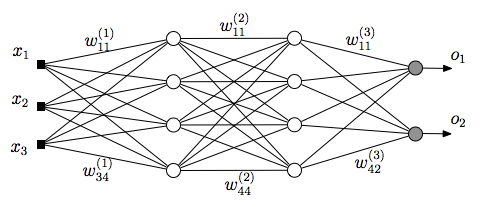
\includegraphics[scale=0.5]{img/MLP}
%     \caption{Paveikslėlio pavyzdys}
%     \label{img:mlp}
% \end{figure}


% \section{Eksperimentinio palyginimo rezultatai}
% % tablesgenerator.com - converts calculators (e.g. excel) tables to LaTeX
% \begin{table}[H]\footnotesize
%   \centering
%   \caption{Lentelės pavyzdys}
%   {\begin{tabular}{|l|c|c|} \hline
%     Algoritmas & $\bar{x}$ & $\sigma^{2}$ \\
%     \hline
%     Algoritmas A  & 1.6335    & 0.5584       \\
%     Algoritmas B  & 1.7395    & 0.5647       \\
%     \hline
%   \end{tabular}}
%   \label{tab:table example}
% \end{table}

\end{document}
